% How to build a tour
\documentclass{beamer}
\usetheme{Madrid}
\usefonttheme{serif}
\usefonttheme{structuresmallcapsserif}
\usepackage{fancyvrb}
\usecolortheme{whale}

\newenvironment<>{varblock}[2][\textwidth]{
    \begin{center}
        \begin{minipage}{#1}
            \setlength{\textwidth}{#1}
            \begin{actionenv}#3
                \def\insertblocktitle{#2}
                \par
                \usebeamertemplate{block begin}}
            {\par
                \usebeamertemplate{block end}
            \end{actionenv}
        \end{minipage}
    \end{center}
}

\begin{document}

\title{Google Earth Tour Building}
\subtitle{For fun and profit}
\author{Joshua Tolley}
\institute{End Point Corp.}

\frame{\titlepage}

\begin{frame}{Whither the Data?}
    Everyone has geographic data
    \begin{itemize}
        \item Who browsed my website, from where? (GeoIP)
        \item Where do I ship most of my orders
        \item What, in fact, are the migration patterns of African and European swallows?
    \end{itemize}
    \begin{varblock}[0.9\textwidth]{Universal Truth}
        Although you may have geospatial data, those data may be uninteresting.
    \end{varblock}
\end{frame}

\begin{frame}{Getting Started}
    The process is pretty simple:
    \begin{itemize}
        \item Determine how you want to display the data
        \item Convert data to latitude and longitude (called ``geocoding'', this is often the most difficult part)
        \item Write a script to loop through the data points and display them (or do it by hand, if you're into that\ldots)
        \item Celebrate
    \end{itemize}
\end{frame}

\begin{frame}{What's Google Earth?}
    Google Earth is essentially Google Maps in 3D, on steroids.
    \begin{center}
        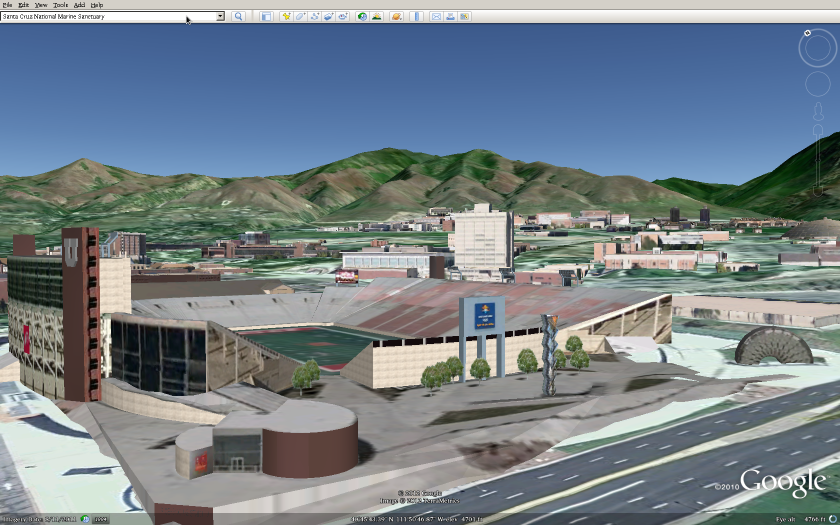
\includegraphics[width=0.8\textwidth]{RiceEcclesStadium-small.png}
    \end{center}
\end{frame}

\begin{frame}{What's Google Earth?}
    \begin{itemize}
        \item Desktop application for Linux (and Mac and Windows, if you insist)
        \item Free, but not open source ;(
        \begin{itemize}
            \item This has caused us some problems, like getting bugs fixed
        \end{itemize}
        \item There exists a paid ``professional'' version
        \begin{itemize}
            \item Allows rendering of video, more flexible editing of large data sets, and a few other things
        \end{itemize}
        \item Also exists in browser plugin form with JavaScript control; ostensibly this works only on Mac and Windows, though we're working to change that
        \item Began as a project by Keyhole software, which Google eventually bought
    \end{itemize}
\end{frame}

\begin{frame}{How to use Google Earth}
    Google Earth accepts files written in Keyhole Markup Language
    \begin{itemize}
        \item XML-based
        \begin{itemize}
            \item Mix between declarative XML, like XML Schema or XML config files, and procedural, like XSLT
        \end{itemize}
        \item Can be created automatically through Google Earth. This is slow and inflexible
        \item Can be written by hand. This is like chewing glass
        \item Can be generated by various helper projects
        \begin{itemize}
            \item Kamelopard: Ruby-based. I wrote most of it, and use it a lot.
            \item PyKML: Python-based. More polished and consistent, but seemingly less capable than Kamelopard
        \end{itemize}
    \end{itemize}
\end{frame}

\begin{frame}{An Example}
    I live on a small farm, where we are growing 12 acres of wheat and raising various poultry. It's here. This is a KML Placemark.
    \begin{center}
        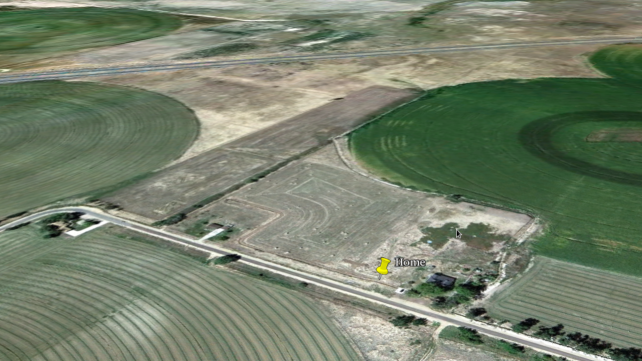
\includegraphics[width=0.8\textwidth]{home-1-small.png}
    \end{center}
\end{frame}

\begin{frame}{An Example}
    These placemarks have descriptions, which can pop up in balloons, like this one. This can include CSS, images, or even Flash video. Icons, text, and balloons can all be styled at will.
    \begin{center}
        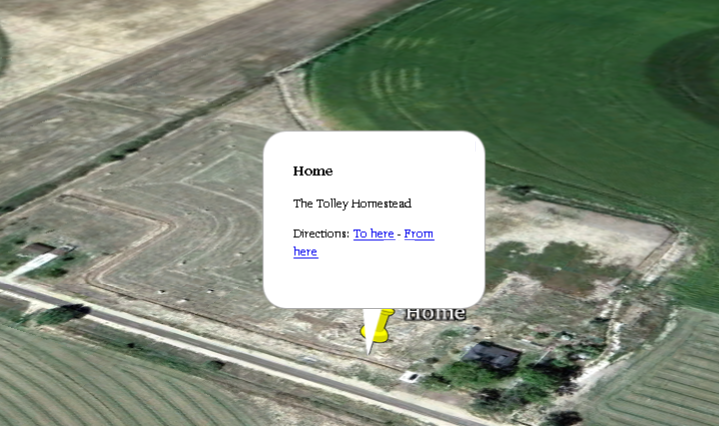
\includegraphics[width=0.8\textwidth]{home-2.png}
    \end{center}
\end{frame}

\begin{frame}{An Example}
    As I said, we're growing wheat this year. This shows the wheat field, outlined with a KML polygon. KML also allows other objects, like lines and 3D models, in various styles.
    \begin{center}
        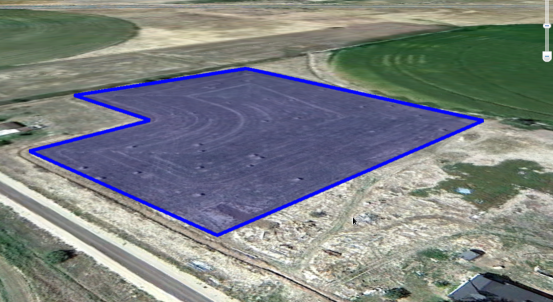
\includegraphics[width=0.8\textwidth]{wheat-small.png}
    \end{center}
\end{frame}

\begin{frame}{An Example}
    Some of these KML objects can include time data
    \begin{center}
        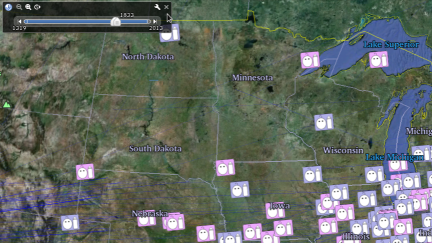
\includegraphics[width=0.8\textwidth]{history-small.png}
    \end{center}
\end{frame}

\begin{frame}{An Example}
    Google Earth allows a few different kinds of added images in a scene,
    called ``Overlays''. This is a Screen Overlay.
    \begin{center}
        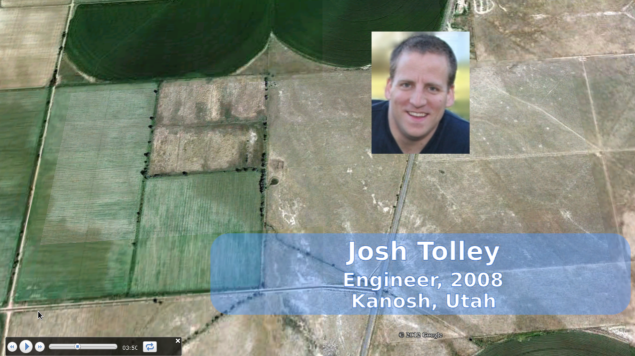
\includegraphics[width=0.8\textwidth]{screenoverlay-small.png}
    \end{center}
\end{frame}

\begin{frame}{An Example}
    Images, placemarks, overlays, etc. call be grouped and animated in a ``Tour''
    \begin{center}
        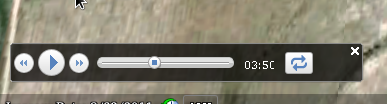
\includegraphics[width=0.8\textwidth]{tourcontrol.png}
    \end{center}
    Tours navigate the viewer automatically, displaying and hiding objects at
    precise locations and for well-defined durations. They can include
    background audio.
\end{frame}

\begin{frame}{More Examples}
    This is useful for more than just pretty pictures.
    \begin{itemize}
        \item Ocean currents
        \item Tsunami shock waves
        \item Wind patterns
        \item Historical events
    \end{itemize}
\end{frame}

\begin{frame}{Liquid Galaxy}
    Google Earth can talk to itself, to broadcast its view of the world. It can
    also receive these packets, and show related views. So if you put multiple
    instances together, you get a panoramic view.
\end{frame}

\begin{frame}{Liquid Galaxy}
    This panoramic view is called a Liquid Galaxy.
    \begin{center}
        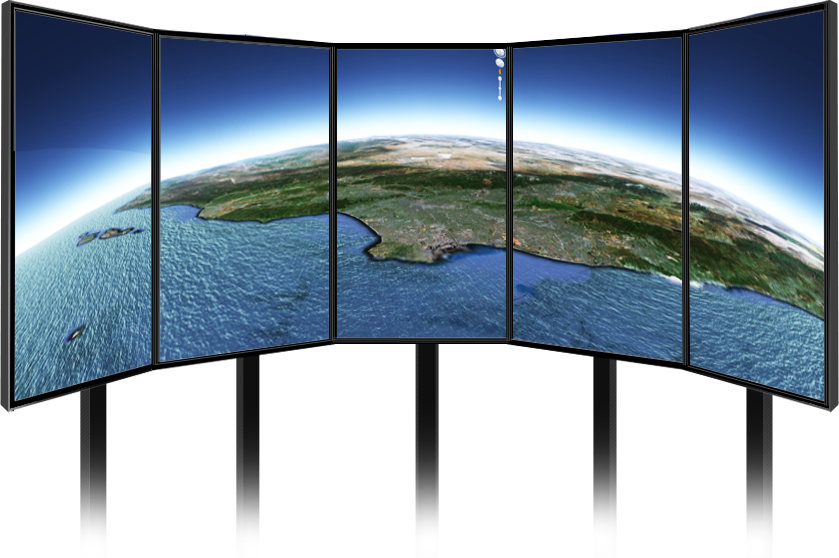
\includegraphics[width=0.8\textwidth]{homepage-globe.png} \\
    \end{center}
\end{frame}

\begin{frame}{Liquid Galaxy}
    End Point has done lots of work with Liquid Galaxies:
    \begin{itemize}
        \item They boot custom ISOs via PXE
        \item Tours and content can be controlled via touch screen
        \item We can monitor and repair galaxies remotely, easily
        \item Tour content can integrate Google Earth with other applications, such as mplayer
    \end{itemize}
\end{frame}

\begin{frame}{Making tours}
    \begin{varblock}[0.9\textwidth]{Universal Truth}
        Writing XML in significant quantities by hand sucks. Debugging and modifying it later redefines ``suckage''.
    \end{varblock}
\end{frame}

\begin{frame}{Making tours}
    \begin{columns}[c]
        \column{0.3\textwidth}
        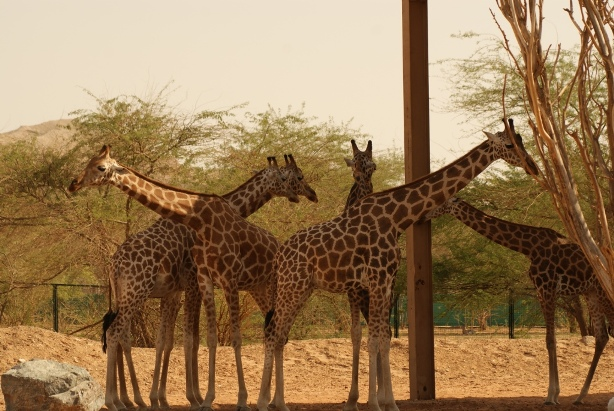
\includegraphics[width=\textwidth]{Al_Ain_Zoo_Giraffe.JPG}

        \column{0.6\textwidth}
        Enter ``Kamelopard'':
        \begin{itemize}
            \item Writes KML for you
            \item Ruby-based, for buzzword appeal
            \item Open source, so you can fix what's broken
            \item Awkward name. It worked for PostgreSQL...
        \end{itemize}
    \end{columns}
\end{frame}

\begin{frame}[fragile]
    \frametitle{Making tours}
    \begin{Verbatim}[fontfamily=courier]
  require 'rubygems'
  require 'kamelopard'
  require 'yaml'

  f = folder 'Tour Resources'
  data = YAML::load_file 'some_data.yml'
  data.each do |d|
    p = point d[:longitude], d[:latitude]
    pl = placemark p, :desc => d[:desc]
    fly_to p, :duration => 4
    f << pl
  end

  write_kml_to 'doc.kml'
    \end{Verbatim}
\end{frame}

\begin{frame}{Kamelopard}
    Kamelopard makes it easy (and succinct!) to generate KML for large data sets.
    \begin{itemize}
        \item Tour of End Point employees, taken straight from employee database
        \item FamilySearch mashup; show ancestral migrations
        \item ``Smart'' power meters' trouble messages vs. lightning strikes
        \item Fisheries' catch records plotted historically, also straight from the database
    \end{itemize}
\end{frame}

\begin{frame}{Large datasets}
    KML can handle large datasets gracefully
    \begin{itemize}
        \item Regions: Data are loaded only when zoomed in close enough
        \item GroundOverlays: Data can be encoded into images that are mapped over the earth
        \item Combining the two, increasingly detailed images or sets of placemarks can appear as the user zooms in closer
        \item DataAppeal creates maps with various models in them, scaling and coloring them based on users' data
    \end{itemize}
\end{frame}

\frame{
    \frametitle{NB! RE: LG}
    There are some important considerations with tours specifically for Liquid Galaxies
    \begin{itemize}
        \item Animations aren't broadcast, so only the master node will animate. Sometimes KML Regions can help mitigate this.
        \item Earth's ViewSync is currently broken. No historical data can be shown
        \item Launching tours is \ldots convoluted. Build an HTML index for your tours.
    \end{itemize}
}

\begin{frame}{So...}
    \begin{itemize}
        \item Google Earth is kinda neat
        \begin{itemize}
            \item (though how might pictures of my backyard help the zombies advance their cause?)
        \end{itemize}
        \item Liquid Galaxies are neat, too
        \begin{itemize}
            \item They can make some pretty pictures
            \item They can also show serious data
        \end{itemize}
    \end{itemize}
\end{frame}

\begin{frame}
    \begin{center}
        Questions?
    \end{center}
\end{frame}

\end{document}
